\documentclass[12pt]{report}
\usepackage{amsmath, amssymb}
\usepackage{listings}
\usepackage[margin=1.6in]{geometry}
\usepackage{fancyvrb}
\usepackage{color}
\usepackage{bussproofs}
\usepackage{pgf, tikz}
\usepackage{graphicx}
\usetikzlibrary{arrows, automata}
\usepackage{hyperref}
\usepackage[scaled=.90]{helvet}
\usepackage{xcolor}
\usepackage{titlesec}
\usepackage[parfill]{parskip}
\usepackage{float}


\DefineVerbatimEnvironment{blockcode}
  {Verbatim}
  {fontsize=\small,formatcom=\color{blue}}

\DefineVerbatimEnvironment{badblockcode}
  {Verbatim}
  {fontsize=\small,formatcom=\color{red}}

\titleformat{\chapter}[display]
  {\normalfont\sffamily\huge\bfseries\color{black}}
  {\thechapter.}{20pt}{\Huge}

\titleformat{\section}
  {\normalfont\sffamily\Large\bfseries\color{black}}
  {\thesection}{1em}{}

\titleformat{\subsection}
  {\normalfont\sffamily\large\bfseries\color{black}}
  {\thesubsection}{1em}{}

\titleformat{\subsubsection}
  {\normalfont\sffamily\bfseries\color{black}}
  {\thesubsubsection}{}{}

\newcommand\code[1]{{\color{blue}\texttt{#1}}}

\fvset{%
  fontsize=\small,
  numbers=left
}

\title{\scshape Git Instruction Manual}
\author{Evan Bergeron\\
Sunny Gakhar\\
Nishad Gothoskar\\
Frederick Lee\\
Ziyang Wang
}

\begin{document}
{\sffamily \maketitle }

\tableofcontents
\newpage
\chapter{Introduction}

This is a manual on how to set up Git on your computer and set up a basic Git workflow. We cover installing, setting up, and working with git. Intermediate workflow tips are provided, as are recommendations for popular editor integrations.

This document is intended for users who want to learn Git to use it in a fast-paced setting such as a hackathon. This document is also useful as a reference for experienced Git users who want to refer to some specifc concept or command which they need.

\section{How to use this document}

Complete beginners to \texttt{git} will want to start with chapters 2 and 3. Chapter 4 covers branches; a topic perhaps not essential to basic usage. Readers already familiar with \texttt{git} may find the final chapters helpful in elevating their workflow efficiency.

\newpage
\section{What is Git?}

Git is a version control system designed to be used for working on small and large projects. It can be used for tracking changes between files and coordinating work on project files among multiple people.

\section{Why use Git?}
When you were in school and you had short homework assignments, you would just start them and finish them in a short span of time (not longer than a week). But when you move on to designing and working on bigger projects with other people, there are multiple issues that come into play. Say you are participating in a hackathon and have finalized your idea and distribution of work among the teammates. How do you actually work on the project together? 

Having all of them work on one computer is not optimal. You might have each teammate work on his own piece independently, but how do you merge everyone's work? Moreover, what if two or more teammates work on the same file, but do different modifications unknown to the others? And what if someone wants to explore a different direction to work on, while keeping the original work intact? Enter Git.

\section{Benefits of Git}
\begin{enumerate}
  \item Using Git, if you're working on a project, you can ``commit" the changes you have made and Git will keep track of all your commits. 
  
  \item If you want to explore a new direction of work which you don't want to integrate with your main project just yet, you can create a new branch and work on the branch without disturbing your main project. You can easily switch between multiple branches to work on multiple features, can when the time comes, you can merge with the main branch. 
\end{enumerate}

\chapter{Installing Git}

\section{For Windows}
If you have Windows, one way of installing Git is from this website:

\url{https://git-scm.com/download/win}

The link should look like the following

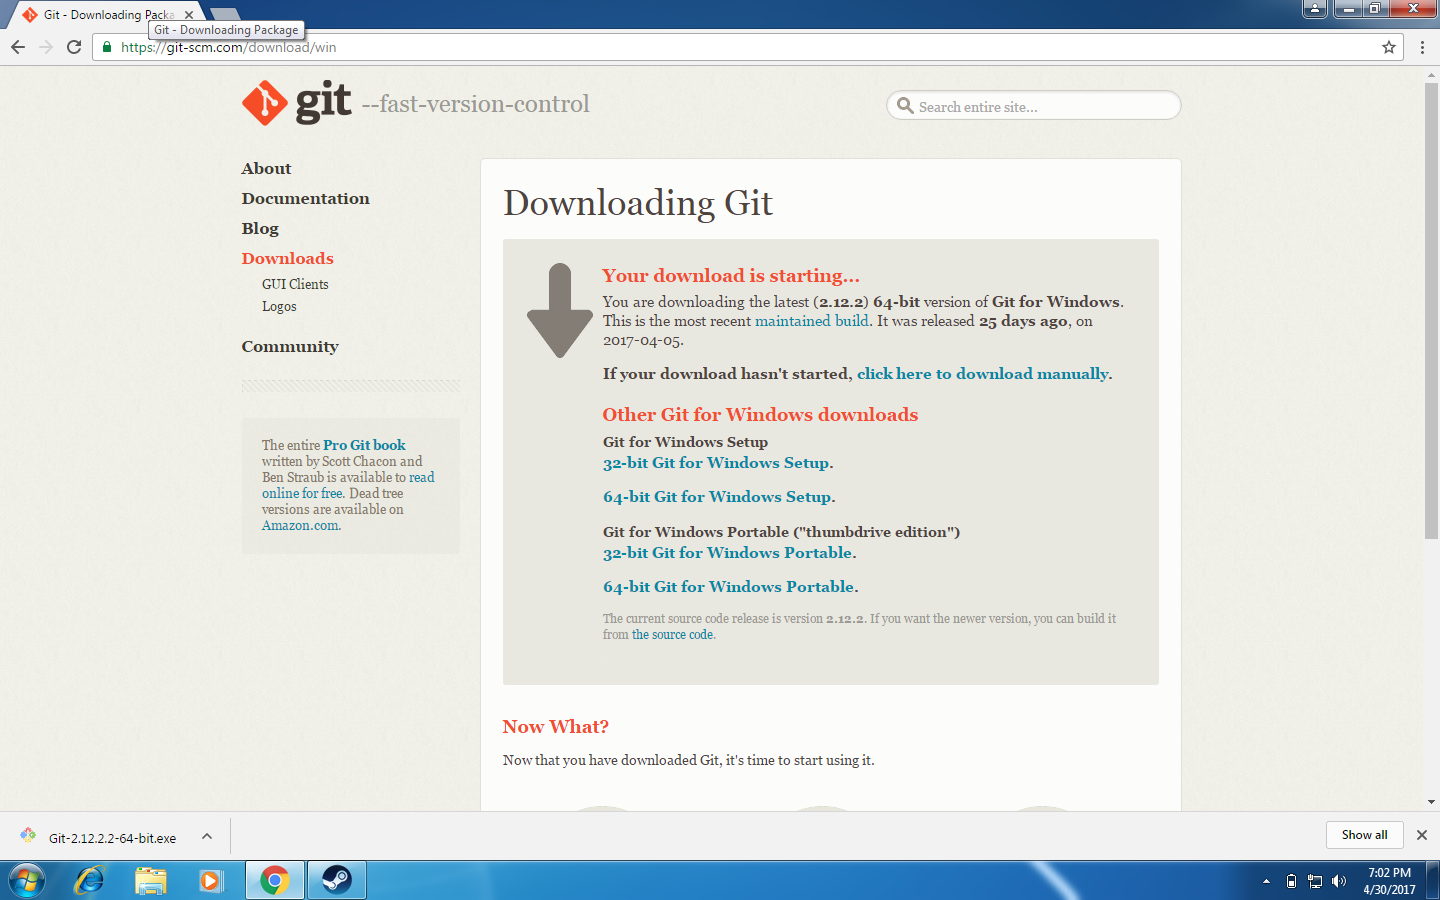
\includegraphics[width=0.75\textwidth]{windows-download.png}

\noindent
Once you have downloaded the installation file, you can open it. 

\textit{Note}: On opening the file, your computer may ask you if you want to run this file as a security warning. Just click Run to run the file.

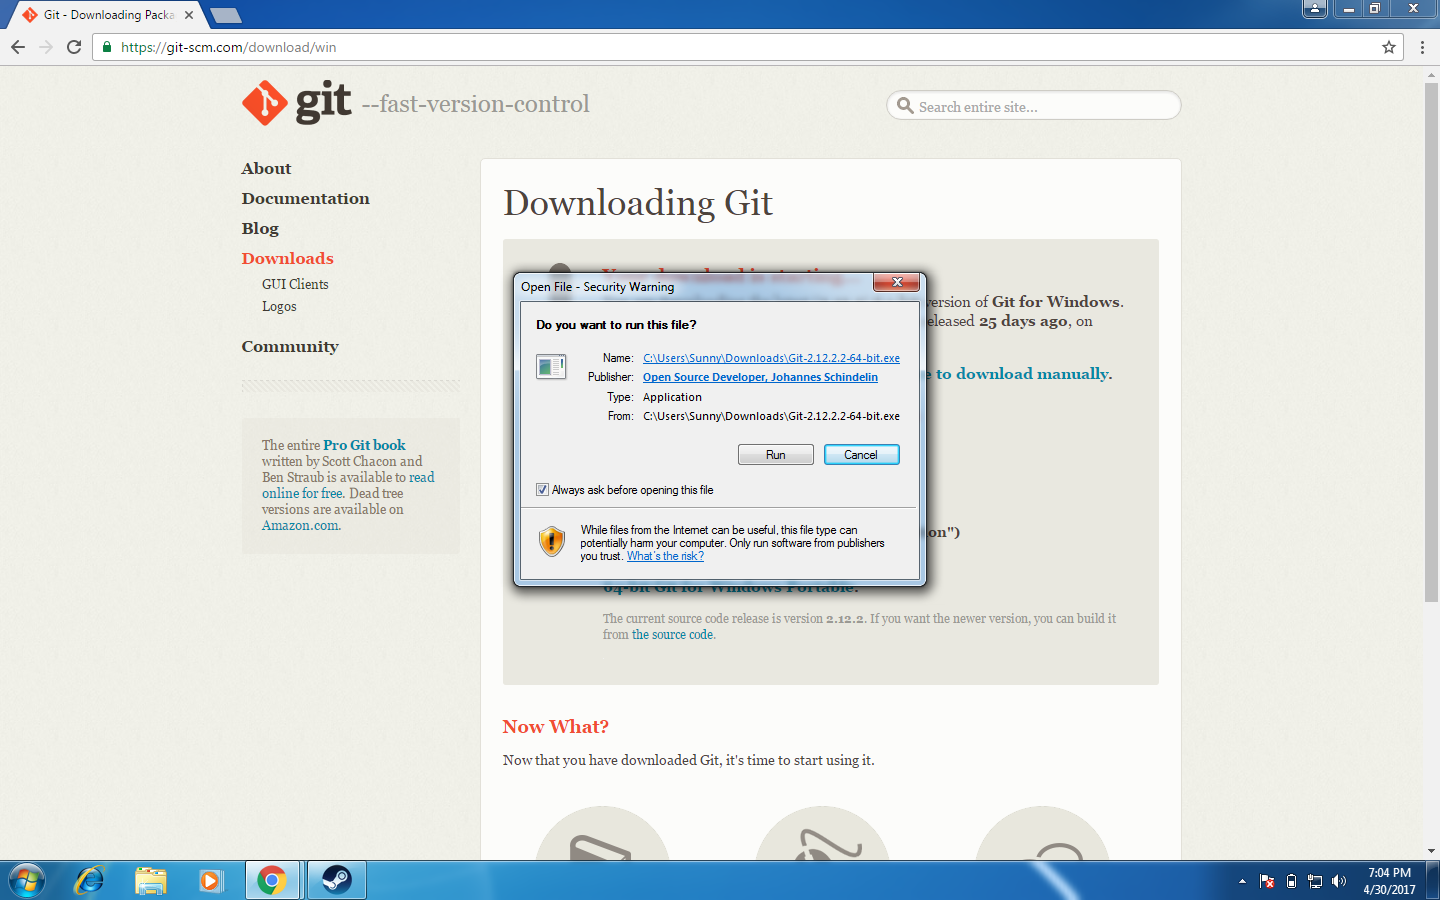
\includegraphics[width=0.75\textwidth]{security.png}

After the security warnings, the installation window should open up. Just follow the steps to install Git on your computer.

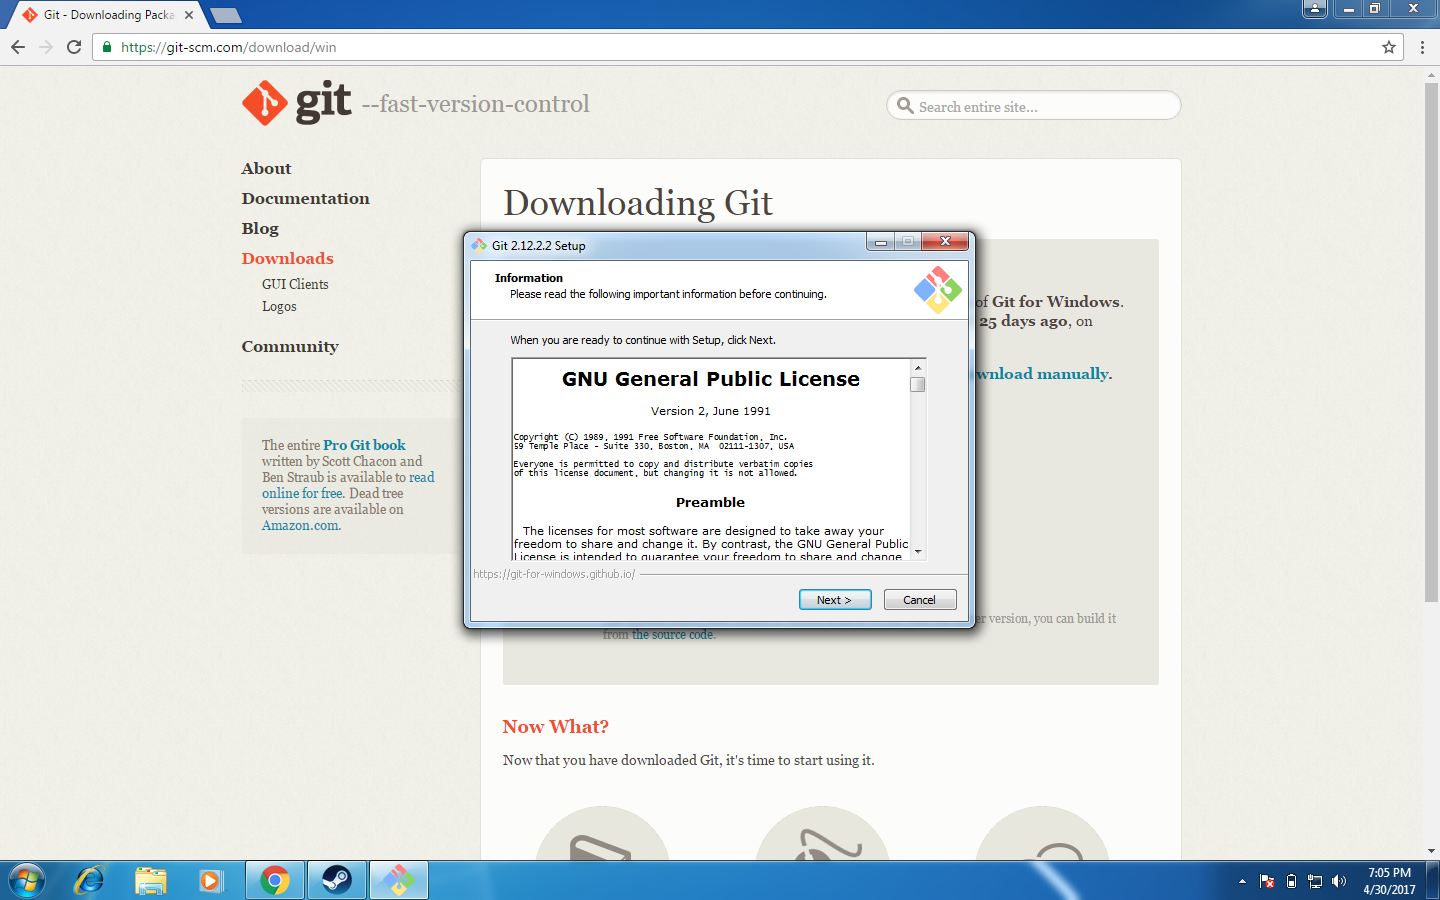
\includegraphics[width=0.75\textwidth]{windows-install.png}

\section{For Mac}

If you have Mac, one way of installing Git is from this website

\url{https://git-scm.com/download/mac}

The link downloads the dmg file i.e. disk image on your computer. Open the disk image.

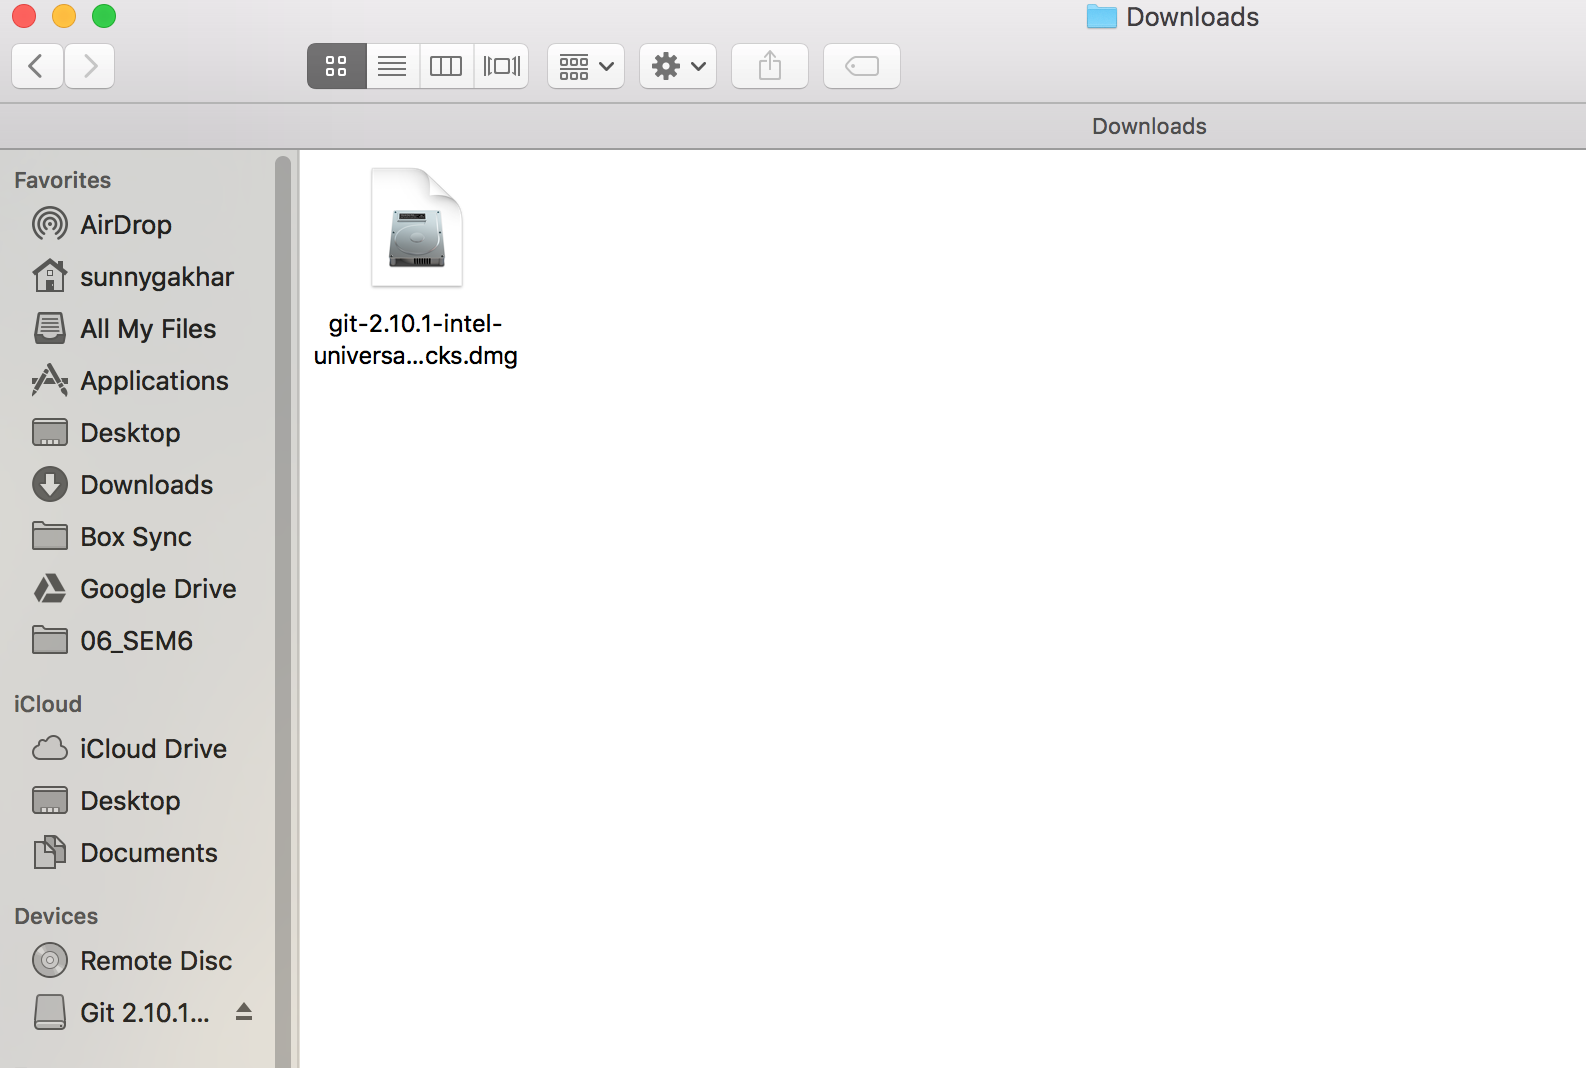
\includegraphics[width=0.75\textwidth]{git-mac-disk.png}

You should be able to see the following. Double click the package to install git. It will open up the installation.

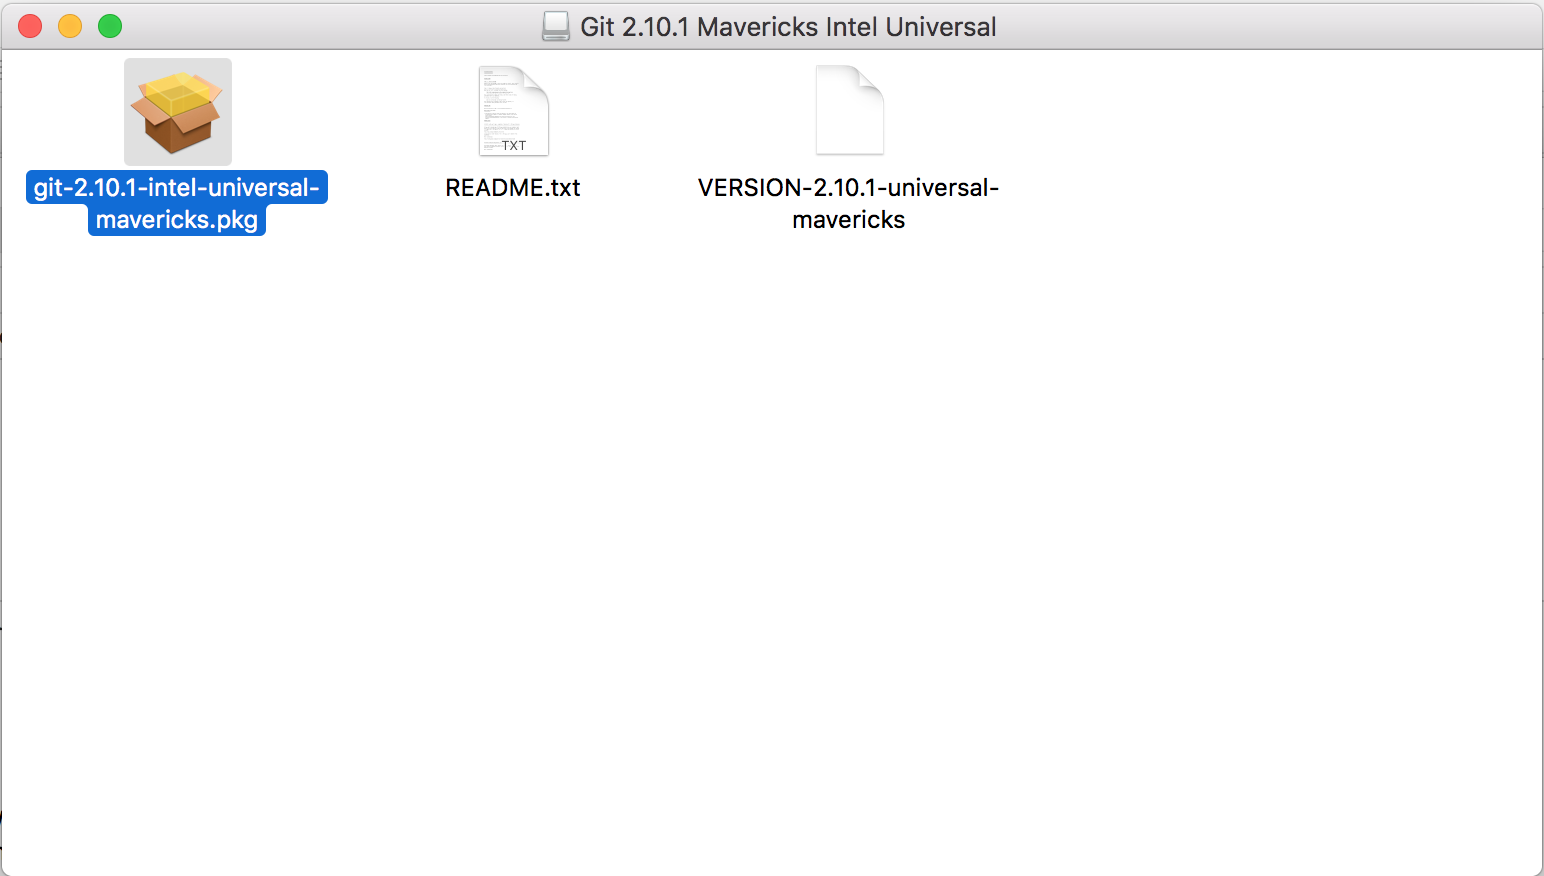
\includegraphics[width=0.75\textwidth]{git-mac-pkg.png}

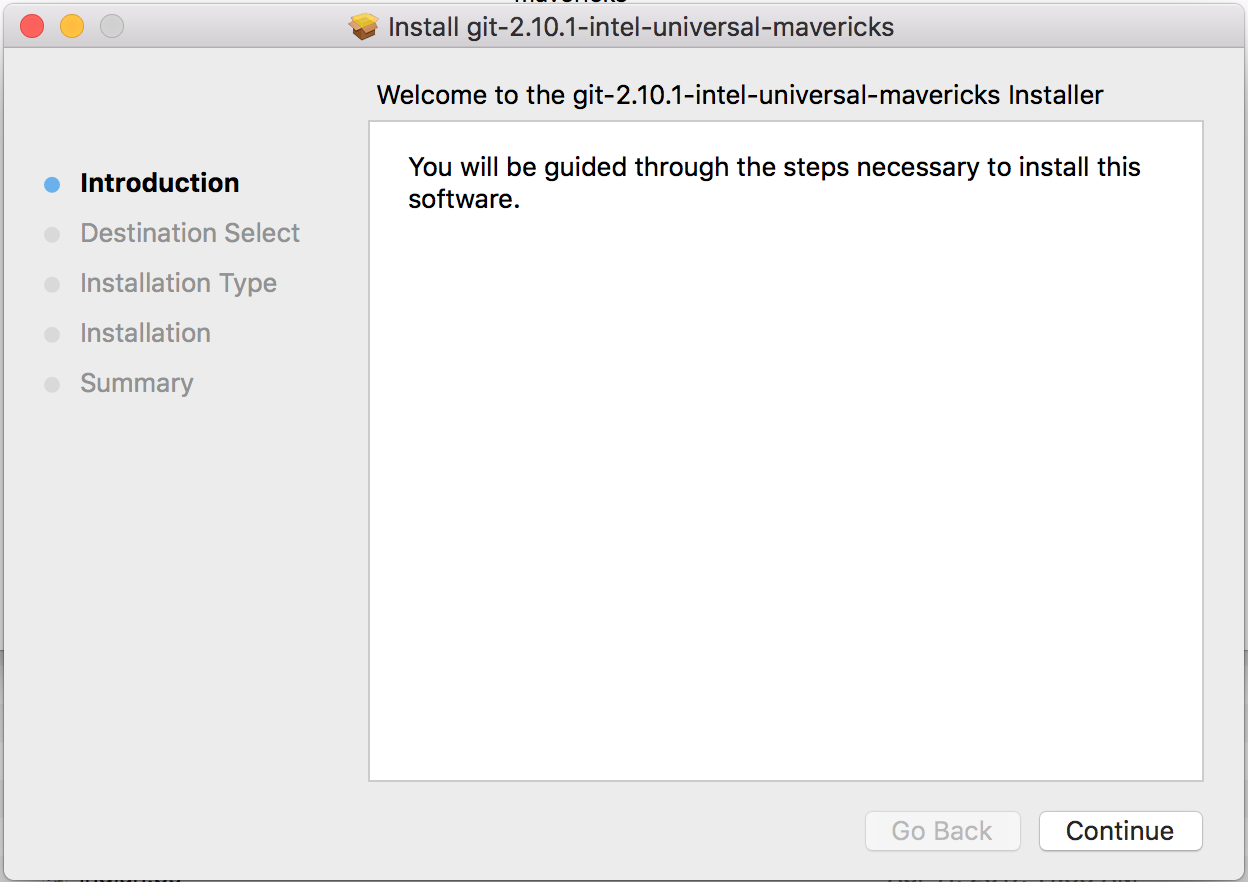
\includegraphics[width=0.75\textwidth]{git-mac.png}

Now just follow the steps to install Git on your machine.

\noindent
Another way of installing Git is using the Xcode Command Line Tools. Open up Terminal 
and simply type \code{git}. If you don’t have Git installed already, it will prompt you to install it.

\section{For Linux}

If you're working on Linux, you can install Git using a basic package management tool that comes with your distribution.

Debian/Ubuntu

\code{\$ apt-get install git}

\bigskip

Fedora

\code{\$ yum install git} (up to Fedora 21)

\code{\$ dnf install git} (Fedora 22 and later)

\bigskip

Arch Linux

\code{\$ pacman -S git}

\bigskip

FreeBSD

\code{\$ pkg install git}

\bigskip

Solaris 9/10/11 (OpenCSW)

\code{\$ pkgutil -i git}

\bigskip

Solaris 11 Express

\code{\$ pkg install developer/versioning/git}

\bigskip

OpenBSD

\code{\$ pkg\_add git}


\chapter{Getting Started}

\section{Crash course on console}

Git is best used with command line interface rather than a graphical interface. Command line interface or console interface is a text interface to your computer. Here we describe how to work with Git on the console (Terminal for Mac/Linux users and Command Prompt for Windows users). We also explain the convention we will be using in this manual to explain Git commands.

\subsection{Windows: Command Prompt}

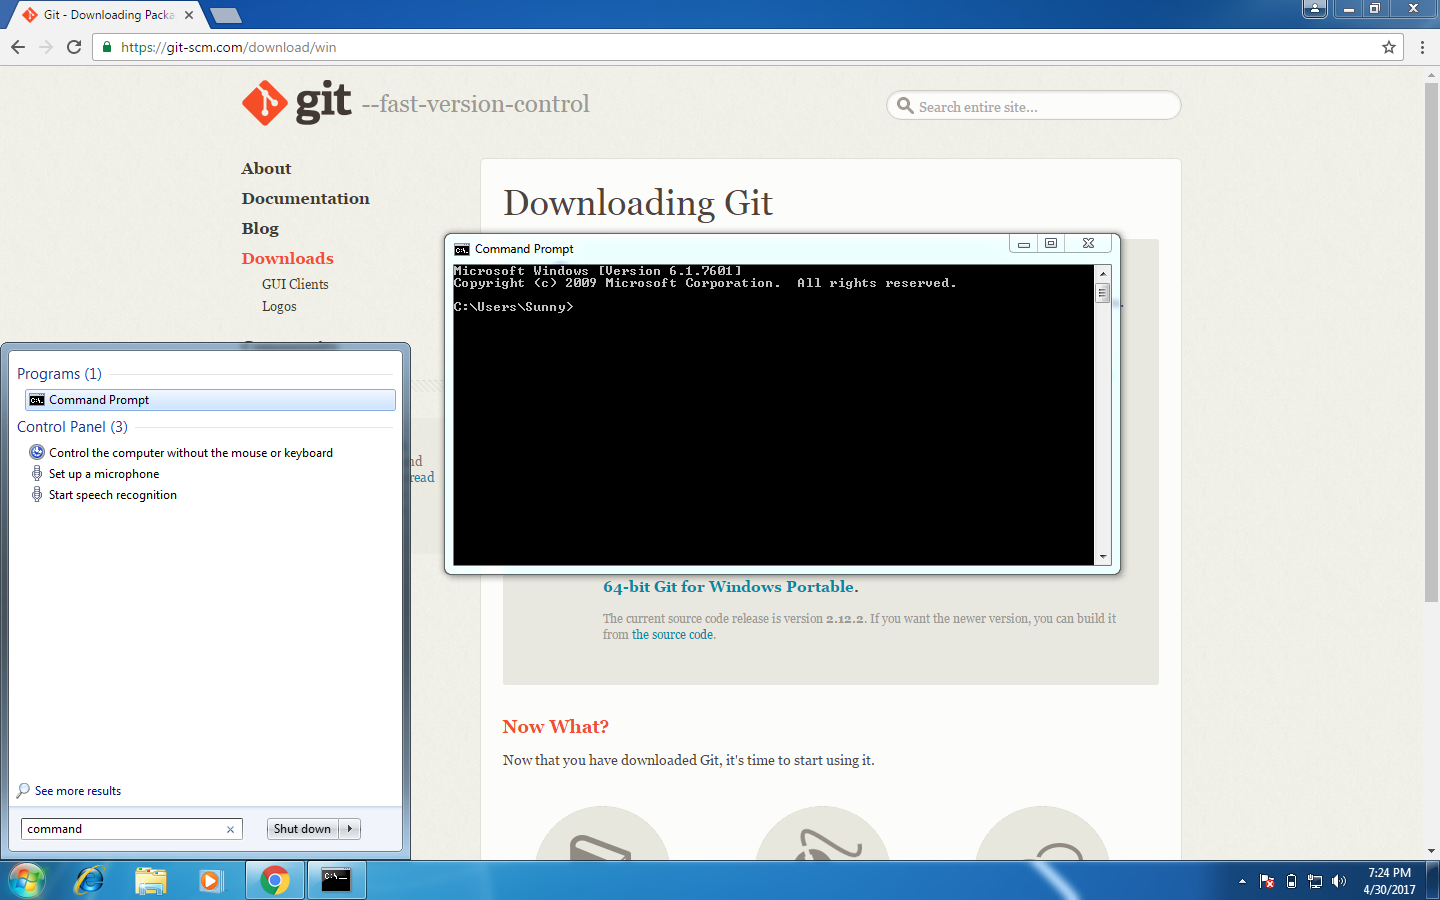
\includegraphics[width=\textwidth]{cmd.png}

The Command Prompt is the default command line on Windows. It can be accessed from the start screen. In Command Prompt you can run commands to open files, go to specific folders, and do other tasks.

\subsection{Mac \& Linux: Terminal}

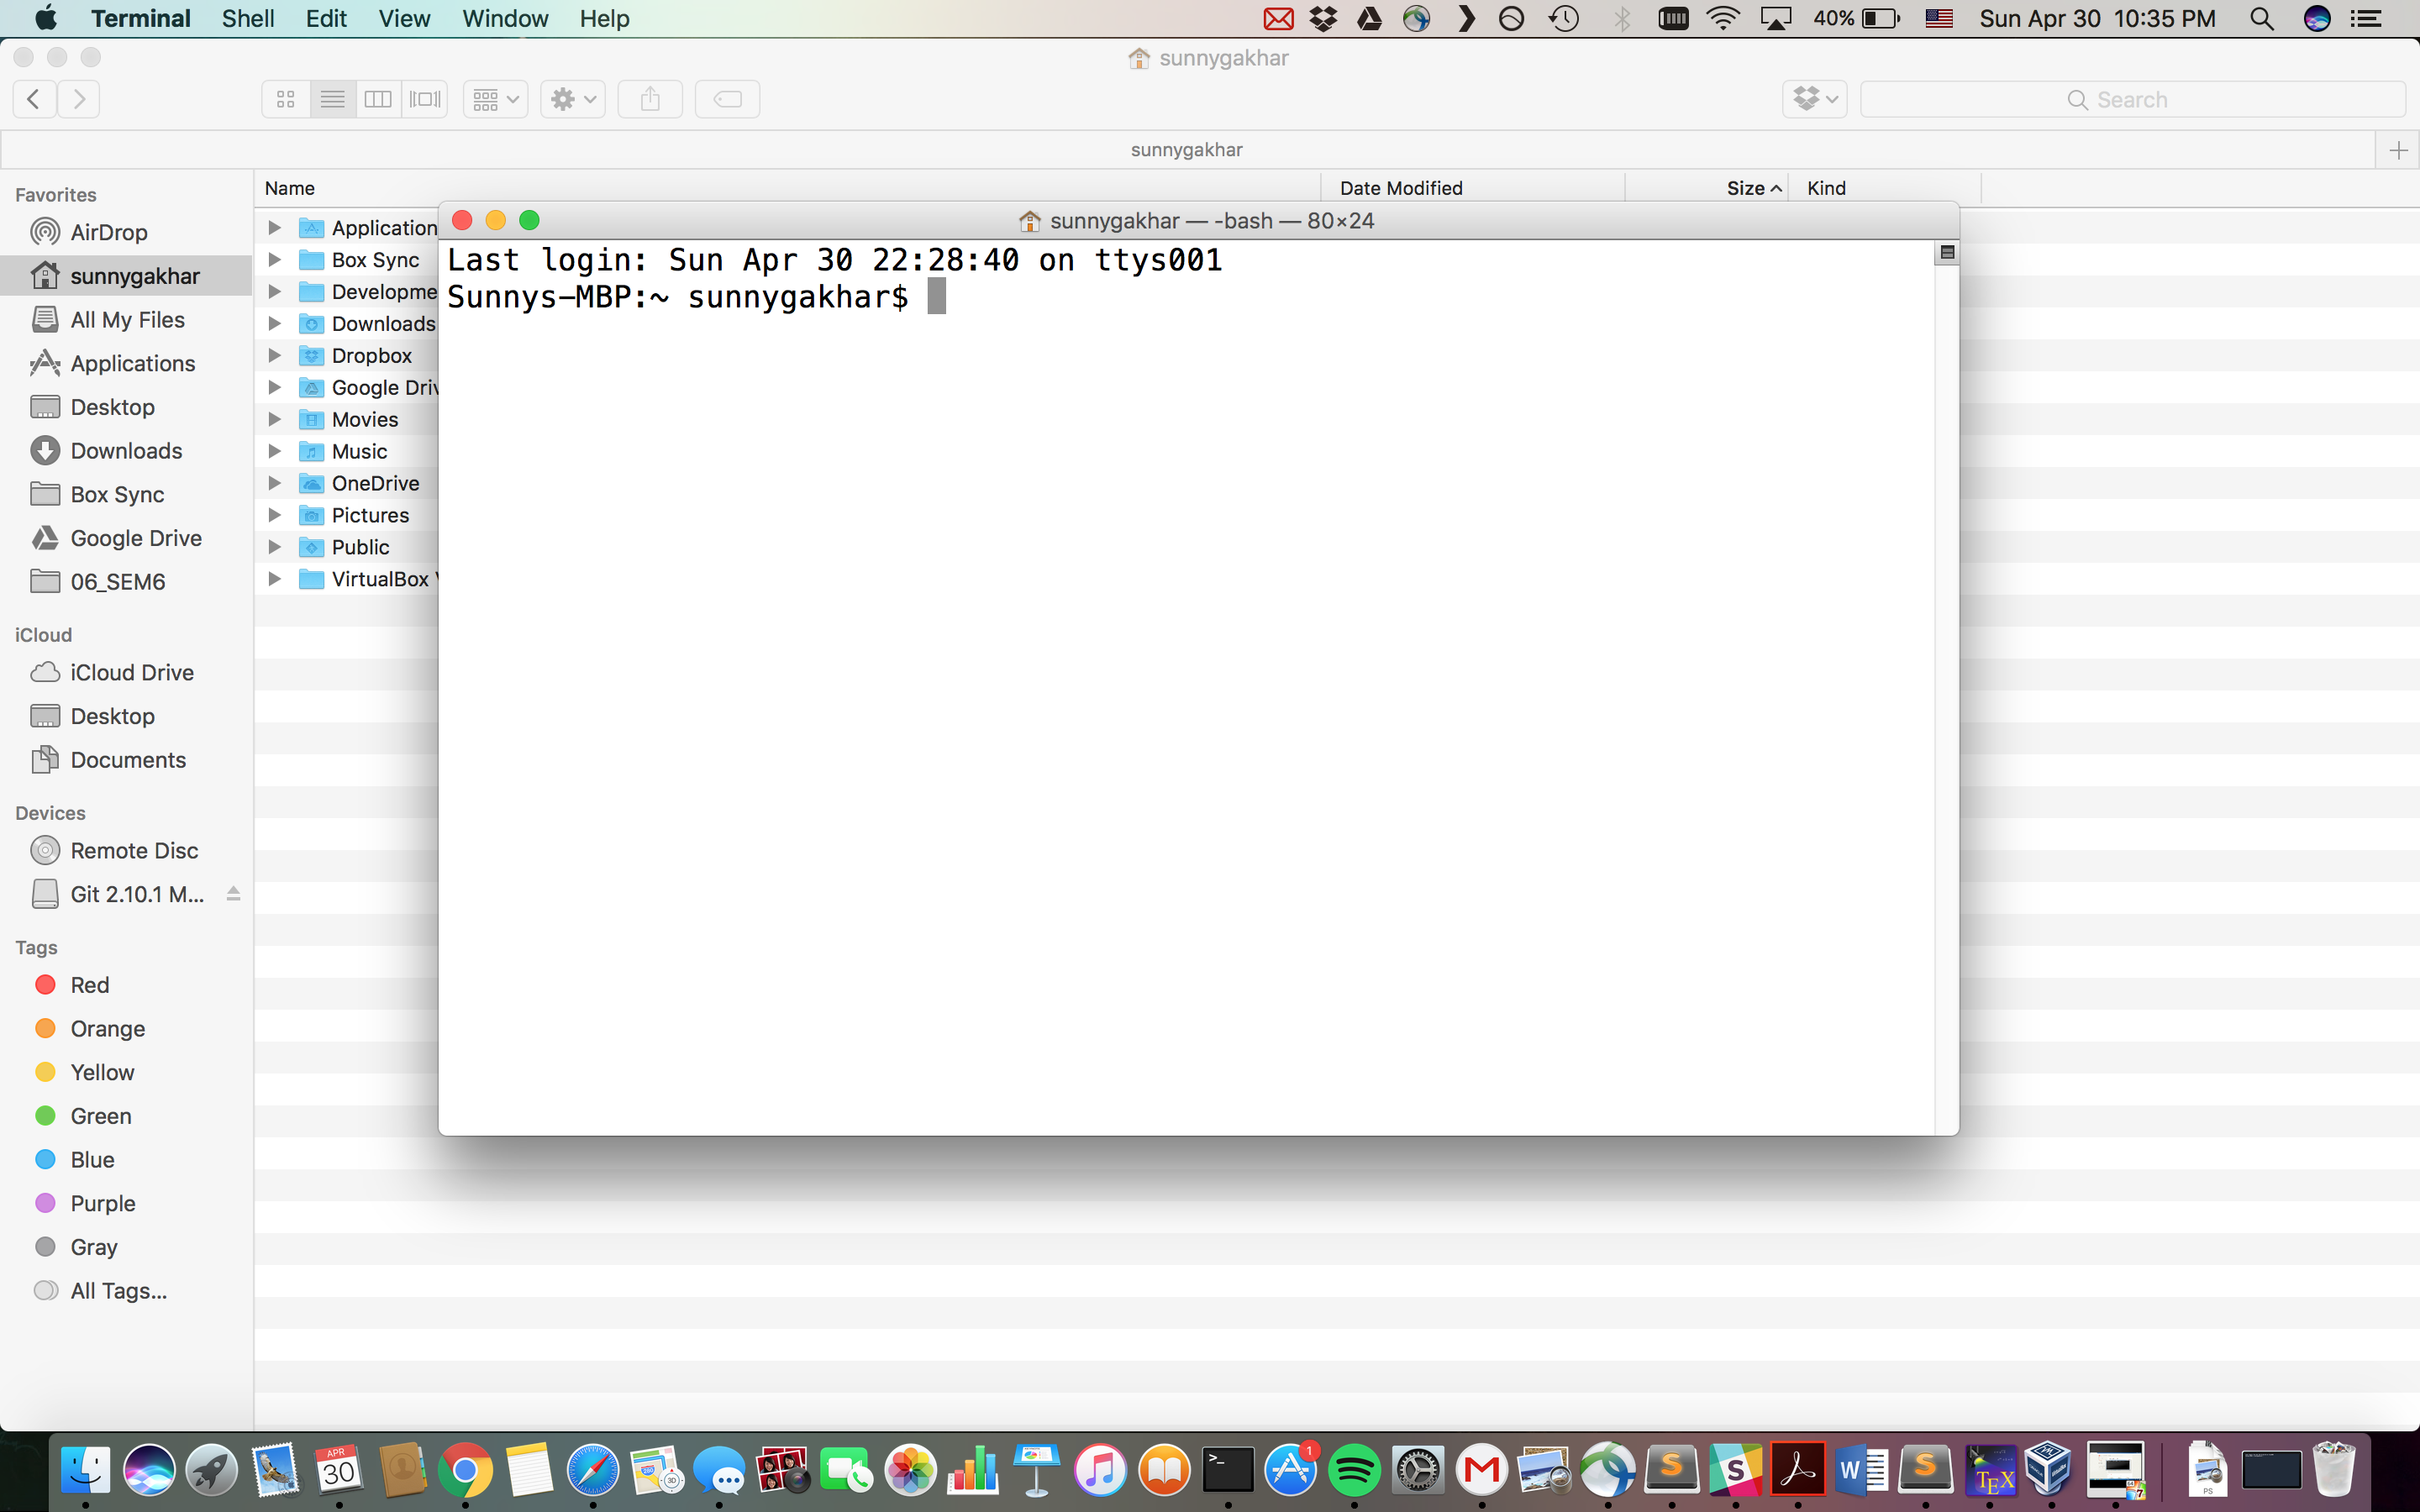
\includegraphics[width=\textwidth]{terminal.png}

Terminal is the default command line for Mac. It is a Unix-based console which can be accessed from Applications. In Terminal you can run commands to open files, go to specific folders, and do other tasks.

\subsection{Convention}

In the rest of this manual, we will describe commands on the command line to use Git. A console command will be written as follows:

\begin{blockcode}
$ pwd
/Users/UserName
\end{blockcode}

Here the \$ denotes the prompt which shows on the console, prompting you to type in a command. Therefore the command here is \code{pwd}. The output of the command is shown on the next line.

To execute the command, type it in the console (Command Prompt/Terminal) and press Enter. 


\section{Initializing a repository}

To make sure you have Git set up, type \code{git} into your console (Terminal for Mac/Linux users and Command Prompt for Windows users) and the following should show up (the full output has been elided here).

\begin{blockcode}
$ git
usage: git [--version] [--help] [-C <path>] [-c name=value]
[--exec-path[=<path>]] [--html-path] [--man-path] [--info-path]
[-p | --paginate | --no-pager] [--no-replace-objects] [--bare]
[--git-dir=<path>] [--work-tree=<path>] [--namespace=<name>]
<command> [<args>]

...

`git help -a' and `git help -g' list available subcommands and some
concept guides. See `git help <command>' or `git help <concept>'
to read about a specific subcommand or concept.
\end{blockcode}
\bigskip
\noindent
To start using Git, we need to create a Git repository. A Git repository contains all the material that you want to track in your project.

To start a new repository for your current directory, type \code{git init} into the console. It should output the following:

\begin{blockcode}
$ git init
Initialized empty Git repository in <path to current directory>/.git/
\end{blockcode}

\bigskip
\noindent
This creates a \code{./git} directory in your current directory, which consists of all information about the repository. It consists of a HEAD file, which points to the current version of the repository.


\section{Adding files to version control}

\subsection*{Problem}

After you edited or created a file, you want to add it to your git repository so that your git recognizes your changes.

\subsection*{Solution}

Use the command:

\code{\$ git add <pathspec>}

\code{<pathspec>} is the path to the file you want to add

\subsection*{Discussion}

The staging environment, or sometimes referred as index, is a file that stores information that you want to edit to the git repository. After you have initialized a repository, you may want to add new files to the repository. However, git does not know which files you want to include in the staging environment. \code{git add} command is used for adding files to the staging environment.

For example, after creating a \texttt{test.txt} file in your working directory, you can check the current status using \code{git status} command. You should get the following message:

\begin{blockcode}
$ git status
On branch master
Untracked files:
  (use "git add <file>..." to include in what will be committed)
  
    test.txt

nothing added to commit but untracked files present
(use "git add" to track)
\end{blockcode}

In order to add the file to the staging environment and notify git for this change, type \code{git add test.txt} and check status. You should get the following message:

\begin{blockcode}
$ git add test.txt
$ git status
On branch master
Changes to be committed:
  (use "git reset HEAD <file>..." to unstage)
  
    New file: test.txt

\end{blockcode}

Now the new file is ready for commit, i.e. ready to be added to the git repository.

If the file you want to add is not in the working directory, use \code{git add <pathspec>} instead to add the file to the staging environment.

\section{Committing changes}

\subsection*{Problem}

You are satisfied with changes you made and you want create a commit to record your changes.

\subsection*{Solution}

To update local repository, use the command:

\code{\$ git commit -m "Message for the commit"}

To update remote repository, use the commands:

\code{\$ git commit -m "Message for the commit"}

\code{\$ git push}


\subsection*{Discussion}

A commit is a record of what files you have added or changed since the last time you committed changes. Running the command \code{git commit -m "Message for the commit"} creates a new commit for all the changes you have made. The message after you creating the commit should contain relevant information about the changed you made.

For example, if you changed some contents in the file \texttt{index.html} and created a new file \texttt{new.txt}, a commit message should look like something as following:

\begin{blockcode}
$ git commit -m "Change index, add new file"
[master 3651e36] Change index, add new file
2 files changed, 10 insertions(+)
create mode 100644 new.txt
\end{blockcode}

The \code{"-m"} flag allows you to give a message without opening a text editor. Alternatively, using \code{git commit} will open your text editor with some message like the following:

\begin{blockcode}
$ git commit
# Please enter the commit message for your changes. Lines starting
# with '#' will be ignored, and an empty message aborts the commit.
# On branch master
# Your branch is up-to-date with 'origin/master'.
#
# Changes to be committed:
# new file:   new.txt
# modified:   index.html
#
~
~
~
".git/COMMIT_EDITMSG" 9L, 283C
\end{blockcode}


If your default text editor is Vim, in order to close Vim, press \code{esc}, then enter \code{":wq"} and press \code{Enter}.

It is worth noting that anything that is still unstaged (files you have created or modified that you haven’t run git add on since you edited them) won’t go into the commit. 

Creating a commit does not change any remote repository. If you are using GitHub, you probably want this commit changes respective contents in the remote repository on GitHub. You can use \code{git push} to update remote repository with committed changes.

\begin{blockcode}
$ git push
\end{blockcode}

\section{Reverting changes}

\subsection*{Problem}

Once you made some changes but you want to undo the changes.

\subsection*{Solution}

\begin{enumerate}
  \item \code{git revert <SHA>}. You have used \code{git push} to change your remote repository, but want to undo the change. You can get the commit hash \code{<SHA>} by \code{git log -n 1}.
  \item \code{git commit --amend}. You created a new commit but have not pushed it to remote repository. There is a typo in your commit message. This command allows you to retype the commit message.
  \item \code{git checkout -- <filename>} You want your files to go back to the state in the last commit.
  \item \code{git reset <SHA>}. You created several commits but have not pushed them to remote repository. The changes you made in the last commit is horrible and you want to go back to certain commit. \code{git reset} rewinds your repository's history back to the specified \code{<SHA>}.
  \item \code{git reflog}. You used \code{git reset} to undo changes, but now you want redo them. \code{git reflog} recovers your directory's history.
\end{enumerate}

\subsection*{Discussion}


One reason people using git as version control is that it can undo changes easily. When you make a new commit, git stores the status of your repository at that specific moment. In the future, you can go back to an earlier version by going back to the status git stored.

\code{git revert <SHA>} command creates a new commit that does the inverse of the given SHA. In other words, it undoes the previous commit by giving opposite changes.

\section{Ignoring files}

\subsubsection*{Problem}

You have one or more files that you do not want Git to keep track of.

\subsubsection*{Solution}

Create a \texttt{.gitignore} file at the base of your Git repository containing the paths of all files that you want Git to ignore.

\subsubsection*{Discussion}

Often you will find that in your projects, you will have files in your repository that do not need to be tracked.  These include automatically generated files, larger libraries that are really external dependencies, or system specific files such as the \texttt{.DS\_Store} file in Macs.

For example, let us have a repository with two files: \texttt{code.py} and \texttt{generated.txt}.  Here we only want to keep track of changes to \texttt{code.py} while ignoring changes to \texttt{generated.txt} which is automatically generated every time \texttt{code.py} is run.

Without a \code{.gitignore} file, running \code{git status} would get the following output:

\begin{blockcode}
$ git status
On branch master
Untracked files:
  (use "git add <file>..." to include in what will be committed)
  
    code.py
    generated.txt

nothing added to commit but untracked files present
(use "git add" to track)
\end{blockcode}

We create a \texttt{.gitignore} file with the following content:

\begin{blockcode}
generated.txt
.gitignore
\end{blockcode}

Running \texttt{git status} again, we see that the generated file and the \texttt{.gitignore} itself are ignored by Git as desired.

\begin{blockcode}
$ git status
On branch master
Untracked files:
  (use "git add <file>..." to include in what will be committed)
  
    code.py

nothing added to commit but untracked files present
(use "git add" to track)
\end{blockcode}

\section{Checking Git history}

\subsubsection*{Problem}

You want to rollback and look at the state of your project at some previous point.

\subsubsection*{Solution}

You can use \code{git log} to look at the commit history and find the commit hash and use:

\begin{blockcode}
$ git checkout 1c0191a6a6264f2e90f6905636321fde897b86df
\end{blockcode}  

This will checkout the previous commit and see the state of the project at that point.

\chapter{Branching}

In git, branching is used to keep track of the different paths of development for your project.  The master branch is the main branch of your project and after features or changes are verified, they are usually added to the master branch of the project.

\section{Creating branches}

\subsubsection*{Problem}

You want to create a new branch (for example if you want a new branch named add\_feature) to begin developing a new component of your project:

\subsubsection*{Solution}

Use the command:
\begin{blockcode}
$ git branch add_feature
\end{blockcode}
  
This creates a new branch in the “development tree”.  Now you can work on this branch of the project without effecting the master branch.
Now in order to bring your current local state to that branch you will have to check it out by running:

\begin{blockcode}
$ git checkout add_feature
\end{blockcode}  

\subsubsection*{Discussion}

The changes you make will be modifying the add\_feature branch rather than the master branch.  To go back to the master branch you will use the same checkout command with master rather than add\_feature. Note that to checkout a different branch your current changes must be committed or stored away before you can switch.

A simple shortcut is to run:

\begin{blockcode}
$ git checkout -b add_feature
\end{blockcode}  

This will create and checkout the new branch add\_feature all in one step.

\section{Deleting branches}

\subsubsection*{Problem}

You are done with development and you want to delete your branch.

\subsubsection*{Solution}

Use the following to delete the branch:
\begin{blockcode}
$ git branch -d add_feature
\end{blockcode}  


\section{Merging branches}

To combine branches, we have two main options: merging and rebasing.

\subsubsection*{Problem}

After working on these separate branch and adding your new feature, you want to merge this work into your master branch so it will persist and new branches can build upon or use the feature you added. 

\subsubsection*{Solution}

 This is what merging does.  It takes a branch and “merges” it into another branch.  This can be done by first checking out the branch you want to merge INTO:

\begin{blockcode}
$ git checkout master
\end{blockcode}  

And then merging the other branch in by:

\begin{blockcode}
$ git merge add_feature
\end{blockcode}

This may happen immediately, unless there are conflicts between the two branches that need to be resolved before they can be successfully merged.  By using git status, you can see in which files these conflicts are located.  Then within the files you will find sections of the form:

\begin{blockcode}
<<<<< HEAD
contents of master
=====
conflicting elements in add_feature
>>>>> add_feature
\end{blockcode}  

And you will have to replace these sections with the content you want and then commit the changes to fully process the merge of the two branches.

\section{Rebasing branches}

\subsubsection*{Problem}

You want to merge your changes from your current branch (which we will call \texttt{feature}) to another branch (which we will call \texttt{master}), but you want your Git history to be more linear than the usual \code{git merge} command with your \texttt{feature} branch's changes applied sequentially after \texttt{master}'s history.

\subsubsection*{Solution}

Update your \texttt{feature} branch's history from \texttt{master} with a \code{git rebase} command by running

\begin{blockcode}
$ git checkout feature
$ git rebase master
\end{blockcode}

and then finally update your \texttt{master} branch with a merge by running

\begin{blockcode}
$ git checkout master
$ git merge feature
\end{blockcode}

\subsubsection*{Discussion}

Rebasing and merging are the two primary ways of combining changes from separate branches with Git.  One primary advantage of rebasing is that the Git history is made more linear which makes it easier to track changes over time.

For example, say that you have been working on a separate branch called \texttt{feature} (shown in blue) on which you have two commits.  At the same time, a friend of yours has committed change \texttt{C} to master (shown in green).

\begin{figure}[H]
\center
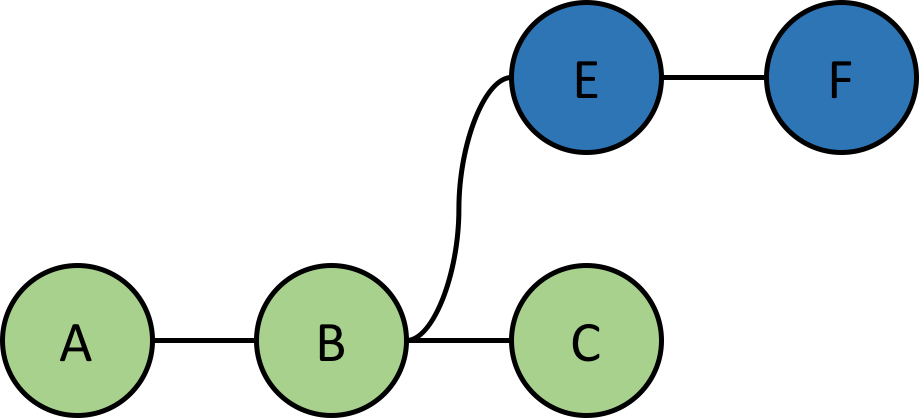
\includegraphics[height=2cm]{feature.png}
\end{figure}

A regular merge command such as
\begin{blockcode}
$ git checkout master
$ git merge feature
\end{blockcode}
would result in the following Git history:
\begin{figure}[h]
\center
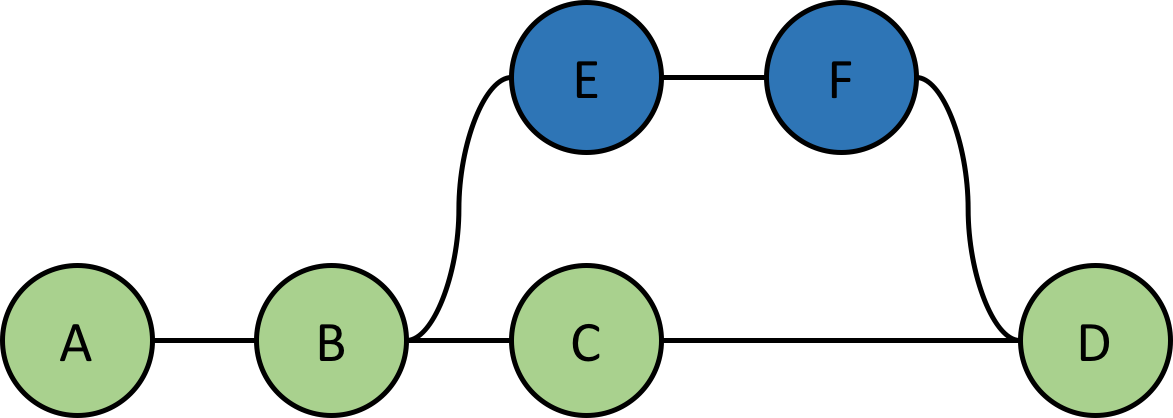
\includegraphics[height=2cm]{merge.png}
\end{figure}

However, the history shown above has the disadvantage of having multiple paths which can make debugging more difficult.  A more linear history would have commits \texttt{E} and \texttt{F} stacked on top of your friend's commits.  To implement this, run the typical rebase command flow via
\begin{blockcode}
$ git checkout feature
$ git rebase master
$ git checkout master
$ git merge feature
\end{blockcode}

The initial rebase command changes the root of your \texttt{feature} branch to your friend's last commit as shown below on the left image.

\begin{figure}[h]
\center
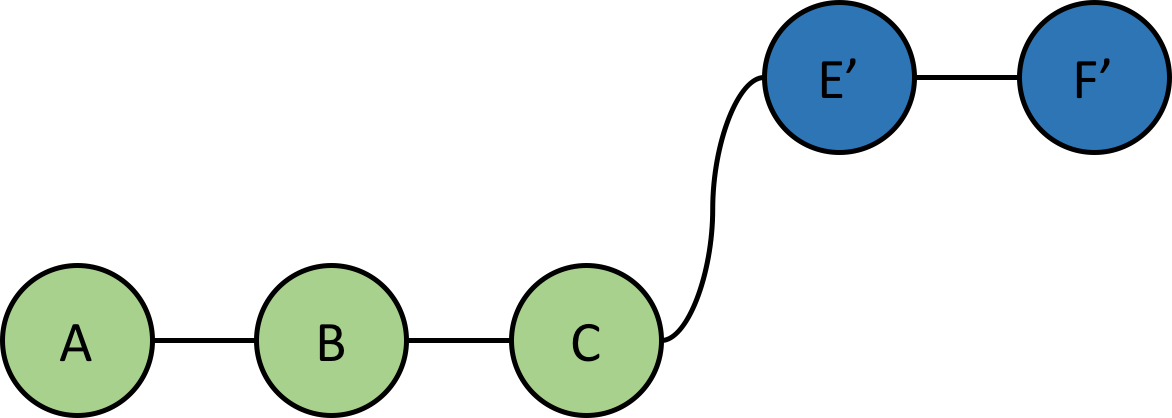
\includegraphics[height=2cm]{rebase.png}
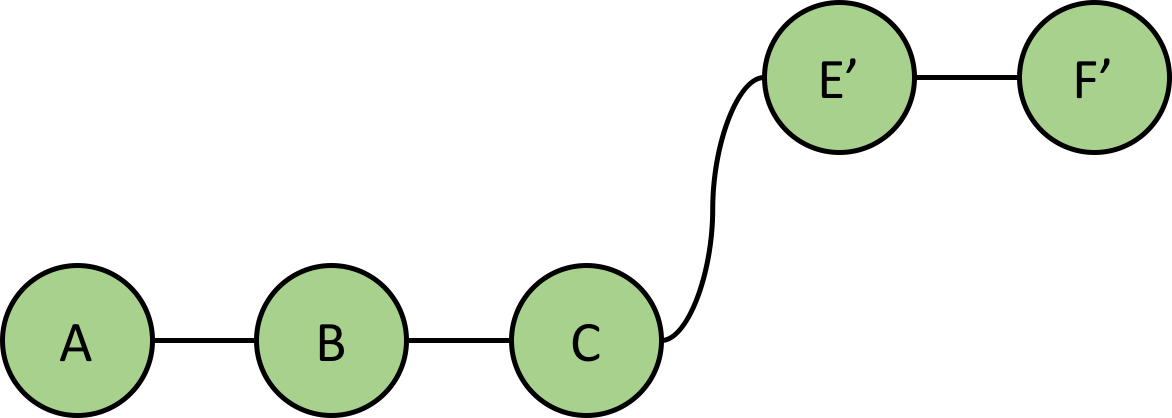
\includegraphics[height=2cm]{rebase_merge.png}
\end{figure}

The final merge of your feature onto master then forwards master's history to match your feature branch as shown above on the right.  As you can see, the history follows a much more linear pattern compared to the branching pattern of a regular merge alone.

\chapter{Intermediate Git}
\section{Cherry-picking commits}

\subsubsection*{Problem}

You have several commits on a separate feature branch, but you only want to apply one or more of these commits to another branch instead of applying all commits.

\subsubsection*{Solution}

Let \texttt{feature} be the branch with the commit you wish to apply, and \texttt{master} be the branch you want to apply these commits to.

First, find the commit-hashes of your desired commits by running:
\begin{blockcode}
$ git checkout feature
$ git log
\end{blockcode}
The commit-hash of your desired commit which may look something like \texttt{f3def414605}.

Then, to apply a single commit to your master branch, run
\begin{blockcode}
$ git checkout master
$ git cherry-pick <commit-hash>
\end{blockcode}

If you have multiple commits you want to commit, for example commits with hashes \texttt{A}, \texttt{B}, and \texttt{C}, you can put multiple hashes onto the same cherry-pick command as shown below:
\begin{blockcode}
$ git checkout master
$ git cherry-pick A B C
\end{blockcode}

\subsubsection*{Discussion}

Cherry-picking is particularly useful when you don't want to apply all changes from a branch to another branch through a merge or rebase, but only want to apply a few specific commits.

For example, take the hypothetical situation where your most recent commit \texttt{F} in your feature branch (shown in blue) is suffering from a application-breaking bug, but your manager wants your changes in commit \texttt{E} to be rolled out by this afternoon.

\begin{figure}[h]
\center
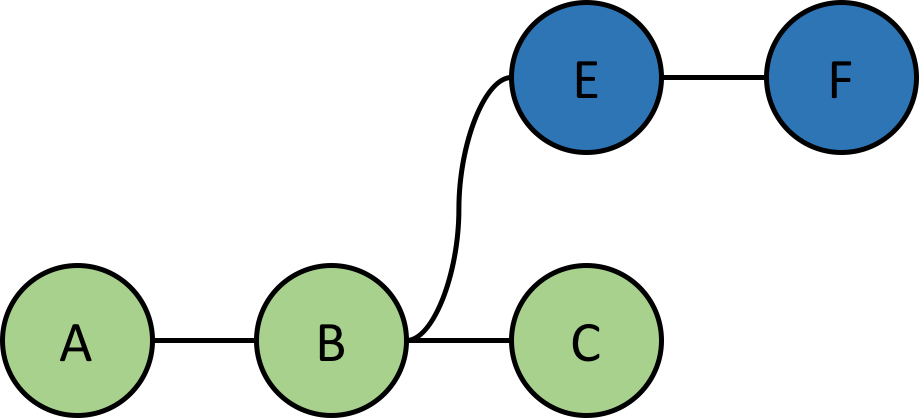
\includegraphics[height=2cm]{feature.png}
\end{figure}

To apply commit \texttt{E} by itself to the master branch (in green), you would first find the commit-hash of \texttt{E} by running \code{git log} and searching for your commit.  A commit-hash is an string of letters and numbers used to uniquely identify commits.  Afterwards, cherry-picking the commit to master gets your final desired result shown below:

\begin{figure}[h]
\center
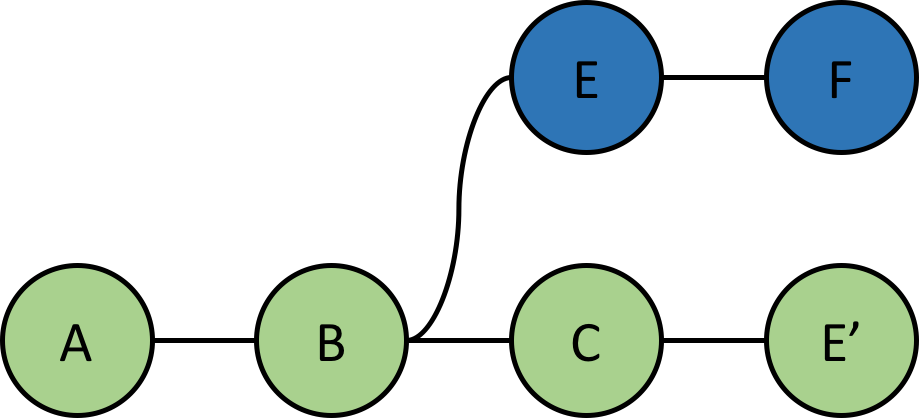
\includegraphics[height=2cm]{cherrypick.png}
\end{figure}

As you can see, commit \texttt{E} through commit \texttt{E'} has been applied to the master branch from your feature branch without merging your entire bug-ridden feature branch to the master branch.  Note that we differentiate \texttt{E} from \texttt{E'} since Git will consider these as two separate and independent commits.

\section{Collaboration with Github}

Github is a website that manages git repositories. You can create an account on the site. Ever user gets an unlimited number of public repositories. Be warned that public repositories can be viewed by anyone accessing \code{github.com}. By default, you retain the copyright to whatever code you post to Github.

You can use github for a more user-friendly version controlling experience.  Almost everything you can do using the command line can be done using the desktop client.  You can easily select files, read their diffs, and commit them.
 
Using the online interface, you can create repositories, add contributors, and track progress very easily.

The workflow using github usually involves many collaborators who make pull requests to the managers of the repository.  Then the manager will approve the pull request, allowing it to merge into the master branch.  Most team collaboration using Github works in this way, making it easy to give feedback and comments on changes before they are finalized and integrated.

The Github Student Development Pack gives many perks including unlimited private repositories as well as discounts on other development tools.  The Development Pack is free for university students.

\section{Easily reordering commits}

\subsubsection*{Problem}
You need to reorder a couple of commits.
\subsubsection*{Solution}
We can simply say:

\begin{blockcode}
$ git rebase -i HEAD~2
\end{blockcode}
This will open an interactive git rebasing session (the \code{-i}
stands for interactive). The window will display something along the
lines of
\begin{blockcode}
pick 370e221 Commit one
pick c342396 Commit two
\end{blockcode}
Simply reorder these lines to reorder the commits.

\subsubsection*{Discussion}

Reordering commits is a common task and can be performed in a single command. 
A naive workflow for this task might look like
\begin{badblockcode}
$ git checkout -b tmp
$ git checkout master
$ git reset --hard HEAD~
$ git cherry-pick tmp
\end{badblockcode}

This works fine, but there’s a simpler method.

\section{Adding partial files}
\subsubsection*{Problem}
You've changed a file, but only want to stage part of the changes to
the file.
\subsubsection*{Solution}
\begin{blockcode}
$ git add -p <file>
\end{blockcode}
This will bring up an interactive prompt. This prompt will cycle
through the different areas of the diff. For each section, you will be
asked if you want to stage each section. You may hit \code{y} or
\code{n} for yes or no.

Once you're done adding the subset of changes you want to commit, you
can double-check you have the right changes staged by saying
\begin{blockcode}
$ git diff --cached
\end{blockcode}
One everything looks good, simply \code{commit} as normal.

\subsubsection*{Discussion}
It can sometimes be helpful to stage only part of the changes made to
a single file. (Especially if there are two logically different
salient tasks). A naive workflow might involve creating separate
branches and manually editing files.


\section{Git aliases}
\subsubsection*{Problem}
You find yourself frequently typing out the same \code{git} commands
over and over. You'd like to save yourself some typing.

\subsubsection*{Solution}

Git aliases are a useful tool to save yourself commonly typed
commands. For instance, we might say
\begin{blockcode}
$ git config --global alias.l "log --oneline"
$ git l
\end{blockcode}
to save ourselves typing out ``\code{log --oneline}'' everytime. It is
worth spending a couple moments to create a handful of shortcuts.

\subsubsection*{Discussion}
It's worth looking online for more detailed commands to add as
aliases. For instance, the following command will display a nicely
formatted ascii graph of all the branches and commits of the
repository:

\begin{blockcode}
$ git log --graph --abbrev-commit --decorate --format=format:' 
  \%C(bold blue)\%h\%C(reset) - \%C(bold green)(\%ar)\%C(reset) 
  \%C(white)\%s\%C(reset) \%C(dim white)- \%an\%C(reset)\%C(bold yellow)
  \%d\%C(reset)' --all
\end{blockcode}
It would be absurd to type this command out in full each time. The
author has this command aliased to \code{g}, so he may simply type
\begin{blockcode}
$ git g 
\end{blockcode}
to achieve the same effect.

\chapter{Vim Integration}

Vim is a popular text editor. Its key feature is called modal editing, which allows users to edit text very quickly. Many professional software developers and professors use vim every day. You should read this chapter if you use vim.

At the time of writing, perhaps the most feature complete vim-git
plugin is Tim Pope’s “vim-fugitive.” Consequently, we will assume
usage of this plugin throughout the entire vim workflows tutorial.

\section{Installing vim-fugitive}

There are a number of ways to install vim-fugitive. The one suggested
by Tim Pope is as follows:
\begin{blockcode}
$ cd ~/.vim/bundle
$ git clone git://github.com/tpope/vim-fugitive.git
$ vim -u NONE -c "helptags vim-fugitive/doc" -c q
\end{blockcode}
Vundle is a great plugin manager for vim -- if you use this, you may
simply add the line
\[
  \code{Plugin 'tpope/vim-fugitive}
\]
to your vimrc and run the \code{PluginInstall} command.

\section{Using vim-fugitive}

\texttt{vim-fugitive} provides a number of functions that wrap common
command line \texttt{git} commands. All of these can be mapped to a
keybinding of your choosing.

\begin{itemize}
\item \code{Glame} opens a vertical split immediately to the left of
  your source code showing the output of \code{git blame}. \code{git
    blame} can be very helpful when browsing a larger codebase,

  A naive solution might first exit vim, manually type “\code{git
    blame <filename>},” then search for the relevant line in the
  resulting output.

\item \code{Ggrep} corresponds to \code{git grep}, a common way to
  search large codebases for keywords. The output opens in another
  buffer, which the authors finds more useful than a separate
  \texttt{tmux} split.

\item \code{Gread} is similiar to \code{git checkout -- <file>}, but
  \code{Gread} operates on a buffer rather than a file. You can use
  \code{u} to undo \code{Gread}, which the authors finds much cleaner
  than dealing with various warnings external to vim.
\end{itemize}

% TODO(Evan) will finish this in a later draft
\chapter{Emacs Integration}

At the time of writing, \code{Magit} is the most feature-complete git
wrapper for emacs. We will thus assume usage of this package.

\section{Installing Magit}
Perhaps the easiest way to install is through MELPA. Just run
\[
  \code{M-x package-install RET magit RET}
\]

\section{Using Magit}
\code{Magit}'s interface is extensive, so cover merely the basics
here. In this section, we adopt the typical \texttt{emacs} key stroke
notation.

\begin{itemize}
\item \code{M-x magit-status RET} opens an interface buffer. \code{n} moves to
  the next item, \code{p} moves to the previous itme. Press
  \code{<TAB>} to expand the selected file. This will open the diff of
  that file.
    
  In the file diff view, \code{git add -p} functionality is readily
  available. Simply while cursor'd over a part of the diff, type
  \code{s} to stage this chunk of the diff.

  When the appropriate chunks have been staged, press \code{c} to
  commit and \code{P} to push.
  
\item \code{M-x magit-log RET master RET} displays an interface log of
  the git repository. \code{magit-log} presents a similar tree
  structure as \code{magit-status}. \code{n}, \code{p}, and
  \code{<TAB>} are used similarly for navigation.
\end{itemize}

\code{q} exits almost any screen in \code{magit}.

\end{document}
